% Timeline
% Demonstrates: horizontal timeline with events, date markers, and styling.
% Compile with: pdflatex main.tex

\documentclass[border=10pt]{standalone}
\usepackage{tikz}
\usetikzlibrary{arrows.meta, positioning}

\begin{document}
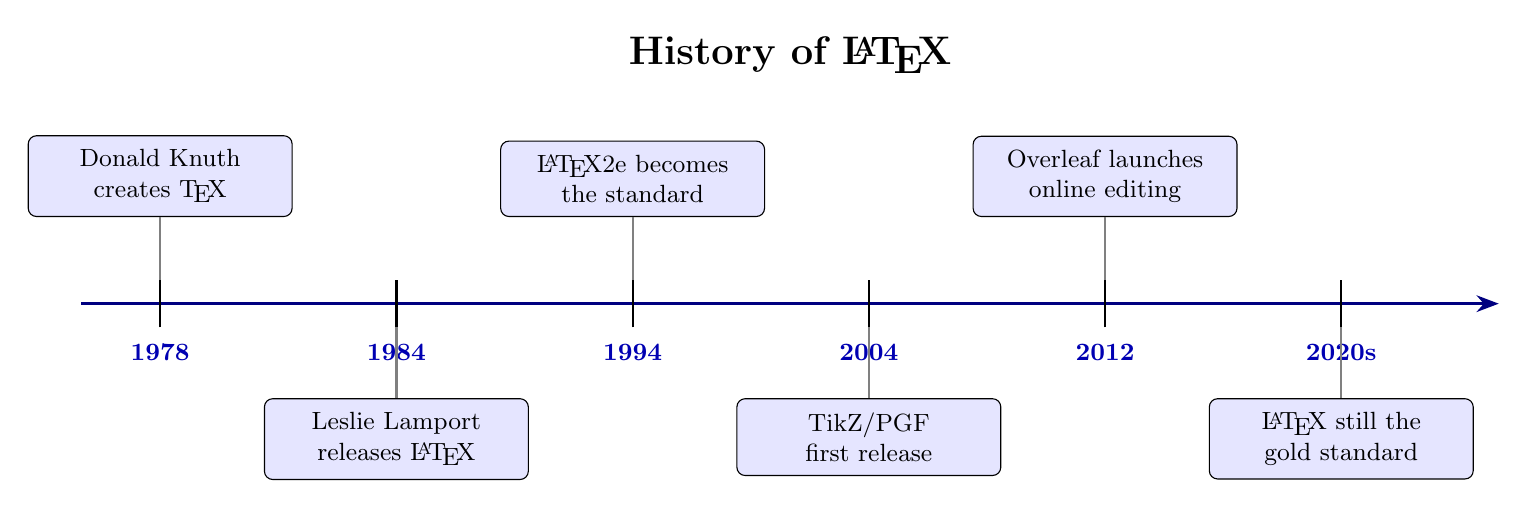
\begin{tikzpicture}[
    event/.style={
        rectangle, rounded corners=3pt, draw=black, fill=blue!10,
        text width=3cm, text centered, font=\small,
        inner sep=5pt,
    },
    year/.style={
        font=\bfseries\small, text=blue!70!black,
    },
]

% --- Main timeline arrow ---
\draw[-{Stealth[length=8pt]}, very thick, blue!50!black]
    (0, 0) -- (18, 0);

% --- Year markers and event boxes ---
% 1978
\draw[thick] (1, -0.3) -- (1, 0.3);
\node[year, below] at (1, -0.4) {1978};
\node[event, above=0.8cm] at (1, 0.3) (e1) {Donald Knuth creates \TeX{}};
\draw[thick, gray] (1, 0.3) -- (e1.south);

% 1984
\draw[thick] (4, -0.3) -- (4, 0.3);
\node[year, below] at (4, -0.4) {1984};
\node[event, below=0.8cm] at (4, -0.4) (e2) {Leslie Lamport releases \LaTeX{}};
\draw[thick, gray] (4, -0.3) -- (e2.north);

% 1994
\draw[thick] (7, -0.3) -- (7, 0.3);
\node[year, below] at (7, -0.4) {1994};
\node[event, above=0.8cm] at (7, 0.3) (e3) {\LaTeX{}2e becomes the standard};
\draw[thick, gray] (7, 0.3) -- (e3.south);

% 2004
\draw[thick] (10, -0.3) -- (10, 0.3);
\node[year, below] at (10, -0.4) {2004};
\node[event, below=0.8cm] at (10, -0.4) (e4) {TikZ/PGF first release};
\draw[thick, gray] (10, -0.3) -- (e4.north);

% 2012
\draw[thick] (13, -0.3) -- (13, 0.3);
\node[year, below] at (13, -0.4) {2012};
\node[event, above=0.8cm] at (13, 0.3) (e5) {Overleaf launches online editing};
\draw[thick, gray] (13, 0.3) -- (e5.south);

% 2020+
\draw[thick] (16, -0.3) -- (16, 0.3);
\node[year, below] at (16, -0.4) {2020s};
\node[event, below=0.8cm] at (16, -0.4) (e6) {\LaTeX{} still the gold standard};
\draw[thick, gray] (16, -0.3) -- (e6.north);

% --- Title ---
\node[font=\Large\bfseries, above=2.5cm] at (9, 0.3) {History of \LaTeX{}};

\end{tikzpicture}
\end{document}
